
\section{概観}

後で詳しく論じるように, この作品は作曲技法の面では4つの楽章間の有機的な動機の結びつきが特徴的である.
しかも, これらの動機はすべて第1楽章の序奏において提示される\footnote{この観点からするとRichard Wagnerの
「ニュルンベルクのマイスタージンガー」と同じ方向を向いているとも言える.}.
各楽章が基本動機に基づいて構築されているという性格のために, 19世紀後半の交響曲としては対位法を愛用するなど, 古典派を思わせる手法が目立っている.
\begin{wrapfigure}{r}{7.0cm}
% \begin{figure}[htbp]
	\centering
	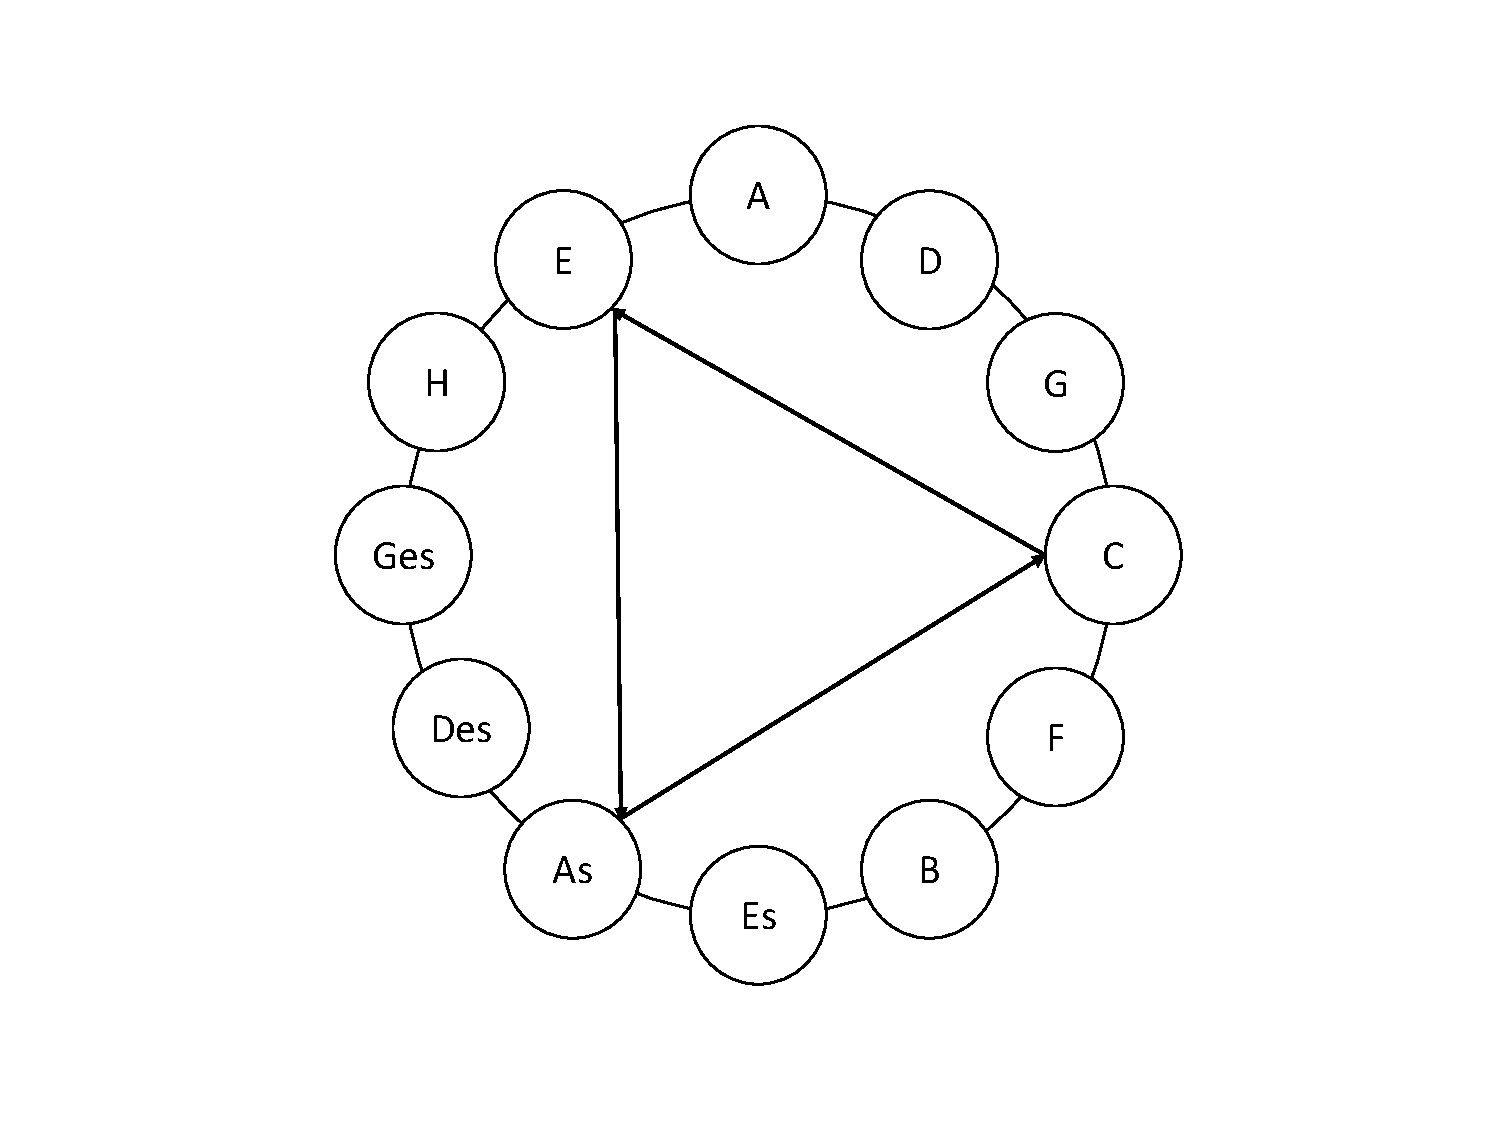
\includegraphics[clip,width=7.0cm]{./figure/modulatory.pdf}
	\caption{第1番の調構造}
	\label{modulatory}
% \end{figure}
\end{wrapfigure}
調性の観点からすると, Brahmsの第1番は彼の多くの作品の中でも独特の立ち位置を占めている:
C-E-As-Cという五度圏上の正三角形を描くような構成 (図\ref{modulatory}) は他にない.
これらの調は互いに遠隔調の関係にあり, いずれも各楽章の最終和音の第3音を起点として自然に移行できる.

第1楽章は大規模な序奏を持つソナタ楽章で, 主部は終始厳格な調子で音楽が展開されるが, コーダで唐突にハ長調に移ると静かに終わる.
これは第2楽章でホ長調へ移るための必然的な要請であるが, 同時に音楽的内容を後続楽章 (特に第4楽章) へ持ち越すための手段ともなっている.
ホ長調の緩徐楽章である第2楽章は, 最終的に三部形式に落ち着いたが, 初演時には現在のものよりも大規模なA-B-A-C-A形式であった.
出版までの演奏を通じてBrahmsはこの楽章をより短く, 圧縮された形へと書き直したのである.
第3楽章は最も短くシンプルな三部形式で, レントラー風のBrahmsらしい間奏曲である.
第4楽章は, やはり大規模な序奏を持つソナタ形式だが, 展開部を欠いており, 再現部が展開部を兼ねる形となっている.
この形式はBrahmsの他の作品にもみられる (弦楽四重奏曲第1番第4楽章など).
また, その序奏にハ短調からハ長調への遷移, アルペンホルンとトロンボーンのコラールという多様な内容が詰め込まれていることも特筆すべきだろう.

曲想, 調性, 構成その他多くの点でこの作品はBeethovenの第5番あるいは第9番と並べて論じられることが多い.
そこでこれら3曲の構成を表\ref{comparison}にまとめておこう.

\begin{table}[htbp]
	\centering
	\begin{tabular}{c|cccc}
		& 第1楽章 & 第2楽章 & 第3楽章 & 第4楽章 \\ \hline
		LvB5 & ソナタ形式 & 変奏曲 & スケルツォ & ソナタ形式 \\
		& c-moll & As-Dur & c-moll & C-Dur \\ \hline
		LvB9 & ソナタ形式 & スケルツォ & 変奏曲 & -- \\
		& d-moll & d-moll & B-Dur & D-Dur \\ \hline
		JB1 & ソナタ形式 & 三部形式 & 三部形式 & ソナタ形式 \\
		& c-moll & E-Dur & As-Dur & C-Dur
	\end{tabular}
	\caption{LvB5, LvB9, JB1の比較}
	\label{comparison}
\end{table}

表\ref{comparison}から明らかなように, これら三曲はいずれも「暗から明へ」という基本的構造は共通であるが,
BrahmsとBeethovenとで中間楽章の調の選び方にはっきりとした相違がある:
Beethovenは中間楽章のどちらか一方は主調である\footnote{Beethovenの場合,
唯一第7番のみA-a-F-Aという調構造であり, (同主調はあるものの) 中間楽章に主調が現れない.}のに対して, Brahmsは (4曲すべての交響曲で) 中間楽章は主調と異なる調性を持つ.
また, Brahmsは中間楽章にBeethoven風のスケルツォを置いていない (第4番のみ第3楽章がスケルツォ風の音楽となっているが, それも2拍子である).

また本作について頻繁に指摘されることとして, 第4楽章第1主題 (譜例\ref{4-62}) がBeethovenの第9番の第4楽章の主要主題 (通称「歓喜の歌」) と類似している.
確かにそうかもしれないが, この指摘にさほど意味はない:
Brahmsのこの主題は全曲の中で必然的にこの形を取ることが決定されており, 他の要因が入り込む余地はない (\ref{sec: mov4}節参照).
加えて, 二つのメロディの類似という現象自体しばしば起こり得る事態であって,
実際この曲についても, 例えばアルペンホルンの主題 (譜例\ref{4-30}) は有名なケンブリッジ大学のグレート・セント・メアリー教会の鐘の音
(日本では「学校のチャイムの音」として知られる) とそっくりである.
他にも, 交響曲第3番第1楽章の第1主題によく似た旋律がRobert Schumannの交響曲第1番第2楽章に現れるなど, この手の事案は枚挙に暇がない.
個々にそのような箇所を指摘して回ったところで, そのような考察から得るものはないだろう.

蛇足であるが, Brahmsの4つの交響曲の調性に関して次の事実に言及されることがある.
これら4曲の調性はC-D-F-Eで, Mozartのジュピター音型に一致する. しかも, Robert Schumannの4つの交響曲B-C-Es-Dを2度平行移動したものでもある.
筆者はこれについて単なる偶然の一致であり意味はないと解釈している:
Brahmsのどの交響曲についても調性はその基本的性格から自然に決定されており, なんらかの意図で選ぶ余地はないように思われる.
特にSchumannの交響曲の番号は単なる出版順であり作曲順は大きく異なっているし, Brahmsもそのことは十分承知していた.
